\documentclass{article}
\usepackage{amsmath}
\usepackage{hyperref}
\usepackage{bookmark}
\usepackage{float} 
\usepackage{soul}
\usepackage{graphicx}
\usepackage{makeidx}
\usepackage[letterpaper, total={7.5in, 10in}]{geometry}

\makeindex
\begin{document}
\title{More Awesome Columb's Law Problems}
\author{Questions, Textbook; Answers, Elias Xu}
\date{January 28, 2025}
\maketitle

\section*{42}
\emph{In the figure below, two tiny conducting balls of identical mass m and identical charge q hand from nonconducting threads of length L. Assume that $\theta$ is so small that $\tan \theta$ can be replaced by its approximate equal, $\sin \theta$. \textbf{(a)} show that $$x = (\frac{q^2 L}{2 \pi \epsilon_0 mg})^{\frac{1}{3}}$$ gives the equilbrium separation x of the balls. \textbf{(b)} is $L = 120 cm, m = 10g, \text{ and } x = 5cm$, what is $|q|$?}
\begin{figure}[H]
    \centering
    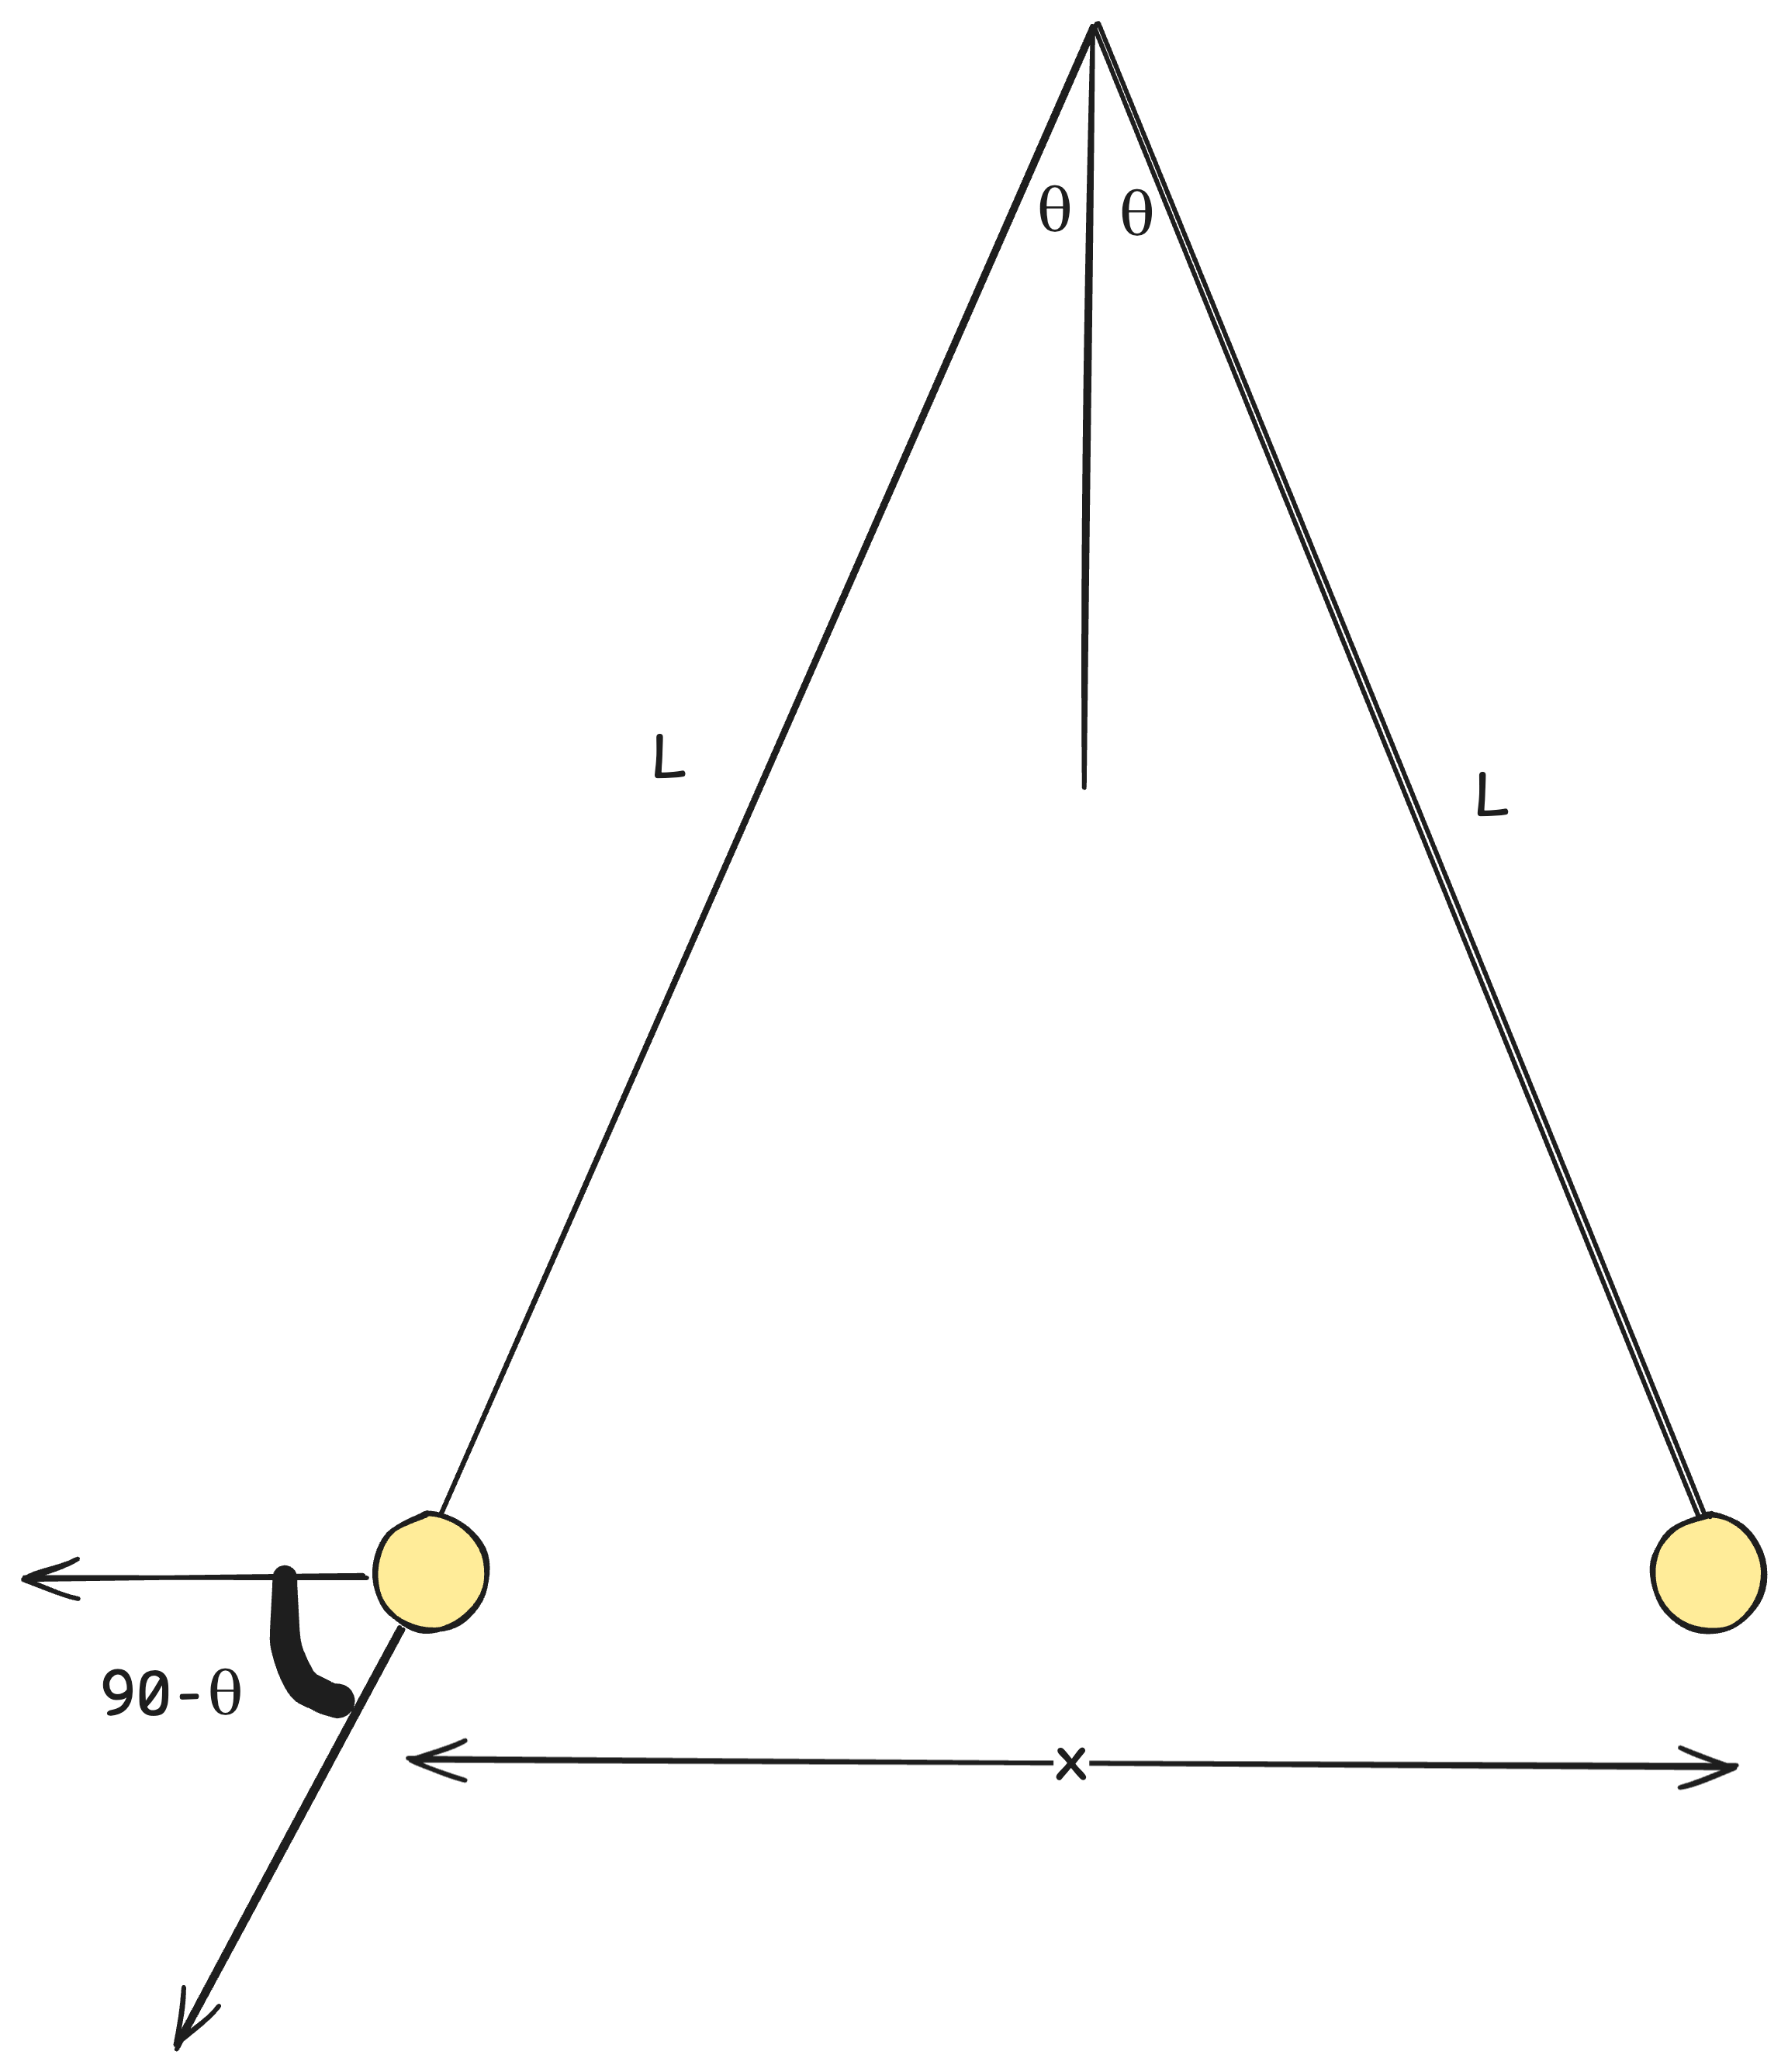
\includegraphics[width=0.4\textwidth]{images/q42.png}
\end{figure}
In the end, this problem is a torque problem with some twists.
$$\sum \tau = 0 = r \times F = I \alpha$$
$$= mgL\sin \theta - \frac{1}{4\pi\epsilon}\frac{q^2L}{x^2} \cos \theta$$
$$g^2 \cos \theta = mg \sin \theta 4 \pi \epsilon x^2$$
Here's we're stuck, except that we can find a relationship between x and L.
$$\frac{\frac{x}{2}}{L} = sin \theta$$
$$x = 2L\sin \theta$$
That means that we can substitute and plug and chug
$$q^2\cos\theta=mg\sin\theta4\pi\epsilon x^2$$
$$q^2 = mg \tan \theta 4 \pi \epsilon x^2 =  mg \sin \theta 4 \pi \epsilon x^2$$
$$q^2 = \frac{2mgx4\pi}{2L}$$
$$\text{\textbf{(a) }} x = \boxed{(\frac{q^2 L}{2 \pi mg\epsilon_0 g})^{\frac{1}{3}} }$$

To solve \textbf{(b)}, we can just plug and chug:
$$q = \sqrt{\frac{x^3\pi\epsilon_0mg}{L}} = \boxed{ \text{ \textbf{(b) }} 2.25\times10^{-8} C }$$

\section*{50}
\emph{The figure below shows a long, nonconducting, massless rod of length L, pivoted at its center and balanced with a block of weight W at a distance x from the left end. At the left and the right ends of the rod are attached small conducting spheres with postive charges q and 2a respectively. At a distance h directly beneath each of these spheres is a fixed sphere with positive charge Q. \textbf{(a)} Find the distance x when the rod is horizontal and balanced. \textbf{(b)} What value should h have so that the rod exerts no vertical force on the bearing when the rod is horizontal and balanced.}
\begin{figure}[H]
    \centering
    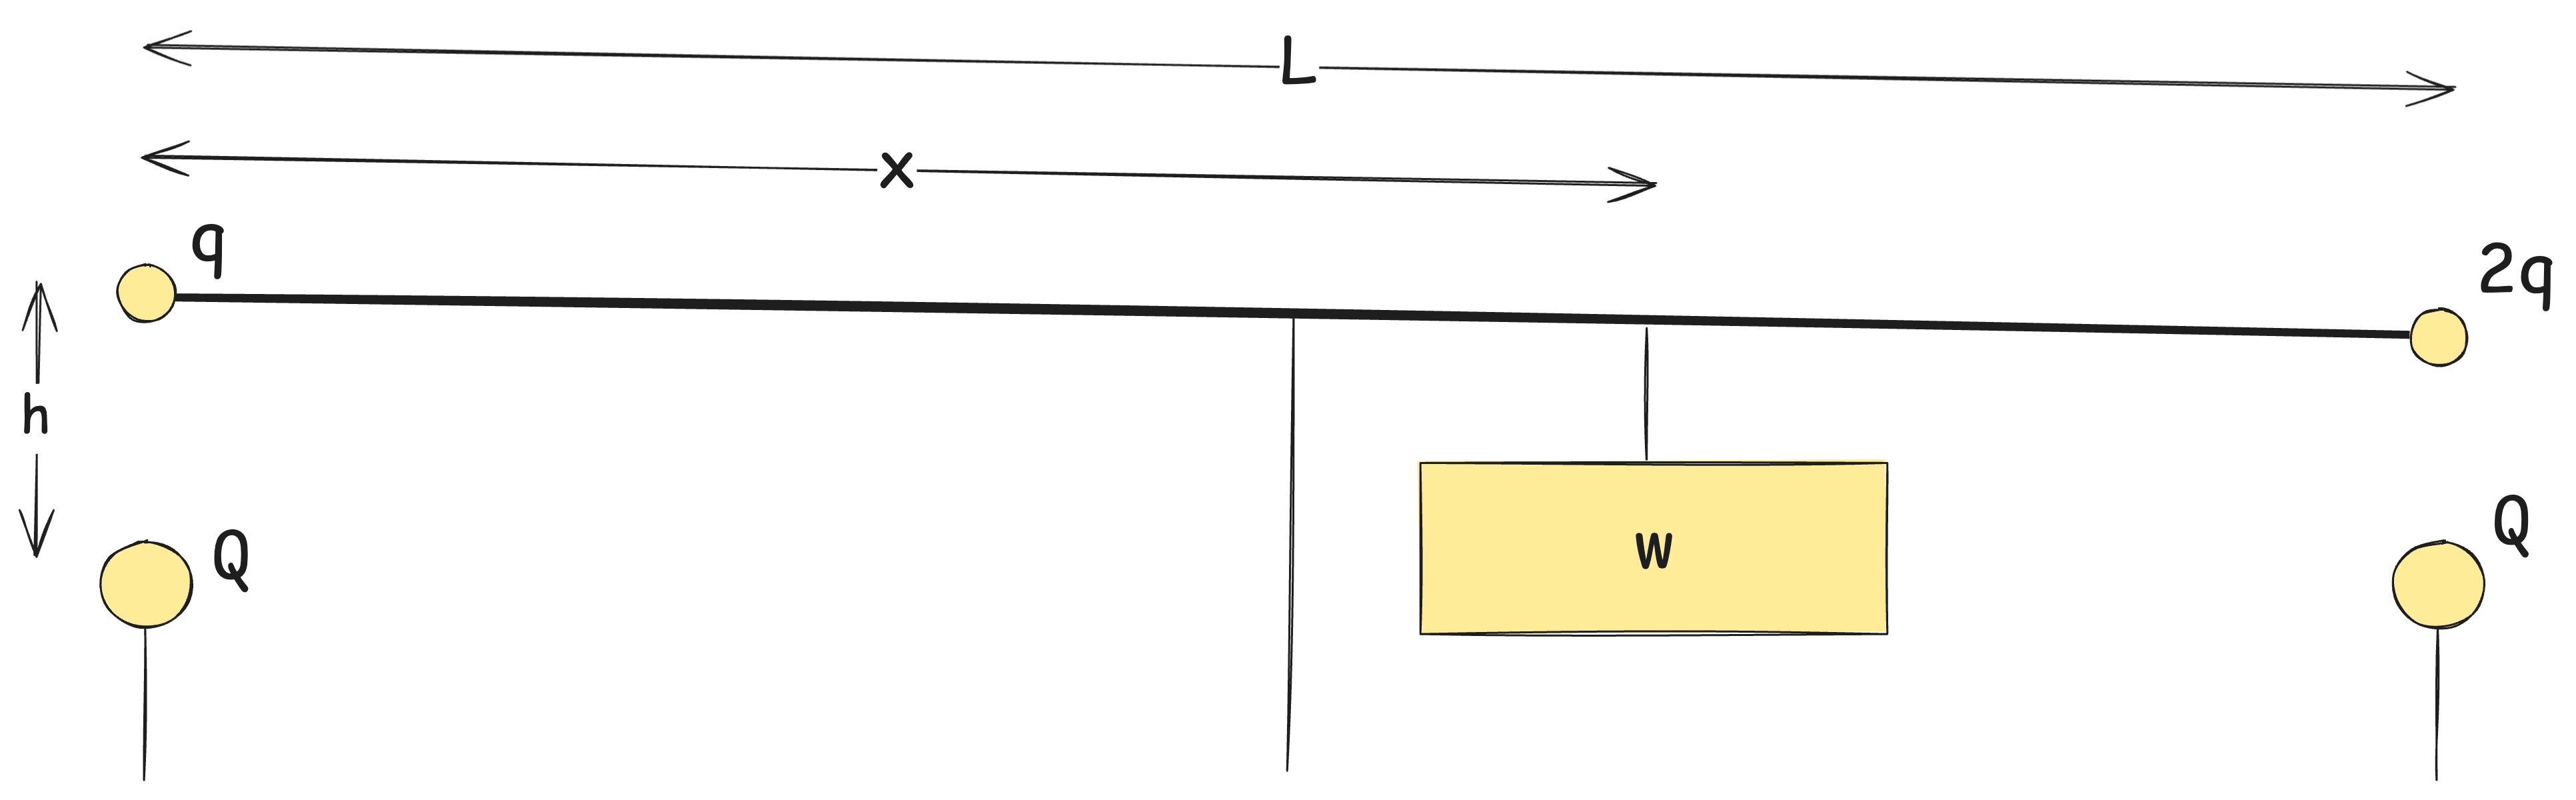
\includegraphics[width=0.4\textwidth]{images/q50.png}
\end{figure}
This is another equilbrium problem, to solve just plug and chug.
$$\sum\tau = 0 = (x - \frac{L}{2})(mg) - F_{c2}\frac{L}{2} + F_c1\frac{L}{2} $$
$$ = 2dmg-\frac{L}{4\pi\epsilon_0}\frac{2qQ}{h^2} + \frac{L}{4\pi\epsilon_0}\frac{qQ}{h^2} \text{[Replace $x - \frac{L}{2}$ with $d$]}$$
$$\frac{LqQ}{4\pi\epsilon_0h^2} = 2dmg$$
$$\frac{LqQ}{wg8\pi\epsilon_0h^2} = d$$
$$\boxed{\text{\textbf{(a)}} \frac{LqQ}{wg8\pi\epsilon_0h^2}  + \frac{:}{2}= x }$$

To find \textbf{(b)} set the sum of forces to zero.
$$\sum F = 0 = F_{c1} + F_{c2} - F_g$$
$$\frac{3qQ}{4\pi\epsilon_0h^2}  = wg$$
$$\boxed{\text{\textbf{(b)}} h = \sqrt{\frac{3qQL}{wg4\pi\epsilon_0}}}$$

\section*{51}
\emph{A charged nonconduction rod, with a length of 2.00 and a cross-sectional area of $4.00 cm^2$, lies along the positive side of an x axis with one end at the origin. The \textbf{volume charge density} of p is charge per unit volumbe in coulombs per cubic meter. How many excess electrons are on the rod if p is \textbf{(a)} uniform, with a value of $-4.00 \mu C/m^3$ or \textbf{(b)} nonuniform, with a value given by $p = bx^2$, where $b = -2.00\mu C/m^5$}\\
\textbf{(a)} is straightfoward multiplication. 
$$V_{\text{cylinder}} = 2m \times 4 \times 10 ^{-4} m^2 = 8 \times 10^{-4} m^3$$
$$p = -4 \times 10 ^-6 C/m^3$$
$$p \times V_{text{cylinder}} = 3.2\times 10^{-19} C = \boxed{\text{\textbf{(a) }}2\times 10^{10} \text{electron}}$$
\textbf{(b)} is slightly more difficult, but it's like integrating a sliced sausage.
$$Q = \int \delta q = \int p \delta V  = \int_0^{2m} bx^2 \delta V$$
Now we have to relate between $\delta V$ and $\delta x$.
$$V = L\times A$$
$$\frac{\delta V}{\delta x} = A$$
$$\delta v = a \delta x$$
Going back to the integration
$$ \int_0^{2m} bx^2 \delta V = \int_0^{2m} bx^2A\delta x = ba \int_{0}^{2} x^2 \delta x$$
$$= -2 \times 10 ^ {-6} \times 4 \times 10 ^{-4} (\frac{x^3}{3}\big|_0^2)$$
$$\boxed{\text{\textbf{(b)} }= 1.33 \times 10 ^ {10} \text{electrons}}$$


\section*{72}
\emph{An electon is project with an initial speed $v_i = 3.2\times 10^5 m/s$ directly toward a very distant proton that is at rest. Because that proton mass is large relative to the electron mass, assume that the proton remains at rest. By calculating the work done on the electron by the electrostatic force, determine the distance between the two particles when the electron instantaneously has speed $2v_i$}\\
To solve, use conservation of energy.
$$ke_i = ke_f + U$$ 
$$mv_i^2 = mv_f^2 - \frac{1}{2\pi\epsilon_0} \frac{q^2}{r} \text{[Multiplied both sides by 2]}$$
$$r = \frac{-\frac{1}{2\pi\epsilon_0} q^2}{mv_i^2- mv_f^2} = \frac{\frac{1}{2\pi\epsilon_0}q^2}{mv_f^2 - mv_i^2} = \boxed{1.64 \times 10 ^{-9} \text{ meters}} \text{ [actual answer was negative but made it positive for funsies]}$$

\end{document}